% 设置 biblatex 额外选项
% \PassOptionsToPackage{gbpub=false, gbtype=false}{biblatex}

% 载入 SJTUThesis 模版
% \documentclass[degree=doctor, zihao=-4, language=english, review]{sjtuthesis}
\documentclass[degree=master, zihao=-4]{sjtuthesis}
% \documentclass[degree=bachelor, openany, oneside]{sjtuthesis}
% \documentclass[degree=course, language=english, openright, twoside]{sjtuthesis}
% 选项
%   degree=[doctor|master|bachelor|course],     % 必选,学位类型
%   language=[chinese|english],                 % 可选(默认:chinese),论文的主要语言
%   bibstyle=[gb7714-2015|gb7714-2015ay|ieee],  % 可选(默认:gb7714-2015),参考文献样式
%   review,                                     % 可选(默认:关闭),盲审模式

% 所有其它可能用到的包都统一放到这里了,可以根据自己的实际添加或者删除。
\usepackage{sjtuthesis}

% 定义图片文件目录与扩展名
\graphicspath{{figures/}}
\DeclareGraphicsExtensions{.pdf,.eps,.png,.jpg,.jpeg}

% 导入参考文献数据库
\addbibresource{bibdata/thesis.bib}

% 信息录入,必须在导言区进行!
% !TEX root = ../thesis.tex

%TC:ignore

\title{上海交通大学学位论文 \LaTeX{} 模板示例文档}
\author{某\quad{}某}
\studentid{0010900990}
\supervisor{某某教授}
% \assisupervisor{某某教授}
\degree{工学硕士}
\major{某某专业}
\department{某某系}
\coursename{某某课程}
\date{2014年12月17日}
% \fund{国家 973 项目 (No. 2025CB000000) \\ 国家自然科学基金 (No. 81120250000)}
\keywords{上海交大, 饮水思源, 爱国荣校}

\entitle{A Sample Document for \LaTeX-based SJTU Thesis Template}
\enauthor{Mo Mo}
\ensupervisor{Prof. Mou Mou}
% \enassisupervisor{Prof. Uom Uom}
\endegree{Master of Engineering}
\enmajor{A Very Important Major}
\endepartment{Depart of XXX}
\endate{Dec. 17th, 2014}
% \enfund{National Basic Research Program of China (Grant No. 2025CB000000) \\
%   National Natural Science Foundation of China (Grant No. 81120250000)}
\enkeywords{SJTU, master thesis, XeTeX/LaTeX template}

%TC:endignore


% 自定义项目标签名称
% \sjtuSetLabel{
%   listfigure = {图\quad 录},
%   listtable  = {表\quad 录}
% }

\begin{document}

% 无编号内容:中英文论文封面、授权页
\maketitle
\makeDeclareOriginality[scans/originality.pdf]
\makeDeclareAuthorization

% 使用罗马数字对前言编号
\frontmatter

% 摘要
% !TEX root = ../main.tex

\begin{abstract*}[zh]
  中文摘要应该将学位论文的内容要点简短明了地表达出来,应该包含论文中的基本信息,
  体现科研工作的核心思想。摘要内容应涉及本项科研工作的目的和意义、研究方法、研究
  成果、结论及意义。注意突出学位论文中具有创新性的成果和新见解的部分。摘要中不宜
  使用公式、化学结构式、图表和非公知公用的符号和术语,不标注引用文献编号。硕士学
  位论文中文摘要字数为 500 字左右,博士学位论文中文摘要字数为 800 字左右。英文摘
  要内容应与中文摘要内容一致。

  摘要页的下方注明本文的关键词(4 \textasciitilde{} 6 个)。
\end{abstract*}

\begin{abstract*}[en]
  Shanghai Jiao Tong University (SJTU) is a key university in China. SJTU was
  founded in 1896. It is one of the oldest universities in China. The University
  has nurtured large numbers of outstanding figures include JIANG Zemin, DING
  Guangen, QIAN Xuesen, Wu Wenjun, WANG An, etc.

  SJTU has beautiful campuses, Bao Zhaolong Library, Various laboratories. It
  has been actively involved in international academic exchange programs. It is
  the center of CERNet in east China region, through computer networks, SJTU has
  faster and closer connection with the world.
\end{abstract*}


% 目录、插图目录、表格目录
\tableofcontents
\listoffigures
\listoftables
\listofalgorithms

% 主要符号、缩略词对照表
% !TEX root = ../main.tex

%TC:ignore

\begin{nomenclature*}
\label{chap:symb}

\begin{longtable}{rl}
  $\epsilon$    & 介电常数 \\  
  $\mu$         & 磁导率 \\
  $\epsilon$    & 介电常数 \\
  $\mu$         & 磁导率 \\
  $\epsilon$    & 介电常数 \\
  $\mu$         & 磁导率 \\
  $\epsilon$    & 电常数 \\
  $\mu$         & 磁导率 \\
  $\epsilon$    & 介电常数 \\
  $\mu$         & 磁导率 \\
  $\epsilon$    & 介电常数 \\
  $\mu$         & 磁导率 \\
  $\epsilon$    & 介电常数 \\
  $\mu$         & 磁导率 \\
  $\epsilon$    & 电常数 \\
  $\mu$         & 磁导率 \\
  $\epsilon$    & 介电常数 \\
  $\mu$         & 磁导率 \\
  $\epsilon$    & 介电常数 \\
  $\mu$         & 磁导率 \\
  $\epsilon$    & 介电常数 \\
  $\mu$         & 磁导率 \\
  $\epsilon$    & 电常数 \\
  $\mu$         & 磁导率 \\
  $\epsilon$    & 介电常数 \\
  $\mu$         & 磁导率 \\
  $\epsilon$    & 介电常数 \\
  $\mu$         & 磁导率 \\
  $\epsilon$    & 介电常数 \\
  $\mu$         & 磁导率 \\
  $\epsilon$    & 电常数 \\
  $\mu$         & 磁导率 \\
  $\epsilon$    & 介电常数 \\
  $\mu$         & 磁导率 \\
  $\epsilon$    & 介电常数 \\
  $\mu$         & 磁导率 \\
  $\epsilon$    & 介电常数 \\
  $\mu$         & 磁导率 \\
  $\epsilon$    & 电常数 \\
  $\mu$         & 磁导率 \\
  $\epsilon$    & 介电常数 \\
  $\mu$         & 磁导率 \\
  $\epsilon$    & 介电常数 \\
  $\mu$         & 磁导率 \\
  $\epsilon$    & 介电常数 \\
  $\mu$         & 磁导率 \\
  $\epsilon$    & 电常数 \\
  $\mu$         & 磁导率 \\
  $\epsilon$    & 介电常数 \\
  $\mu$         & 磁导率 \\
  $\epsilon$    & 介电常数 \\
  $\mu$         & 磁导率 \\
  $\epsilon$    & 介电常数 \\
  $\mu$         & 磁导率 \\
\end{longtable}

\end{nomenclature*}

%TC:endignore


% 使用阿拉伯数字对正文编号
\mainmatter

% 正文内容
% !TEX root = ../thesis.tex

\chapter{简介}

这是 \sjtuthesis 的示例文档,基本上覆盖了模板中所有格式的设置。建议大家在使用模
板之前,除了阅读《\sjtuthesis\ 使用文档》,这个示例文档也最好能看一看。

\section{二级标题}

\subsection{三级标题}

\subsubsection{四级标题}

Lorem ipsum dolor sit amet, consectetur adipiscing elit, sed do eiusmod tempor
incididunt ut labore et dolore magna aliqua. Ut enim ad minim veniam, quis
nostrud exercitation ullamco laboris nisi ut aliquip ex ea commodo consequat.
Duis aute irure dolor in reprehenderit in voluptate velit esse cillum dolore eu
fugiat nulla pariatur. Excepteur sint occaecat cupidatat non proident, sunt in
culpa qui officia deserunt mollit anim id est laborum.

\section{脚注}

Lorem ipsum dolor sit amet, consectetur adipiscing elit, sed do eiusmod tempor
incididunt ut labore et dolore magna aliqua. \footnote{Ut enim ad minim veniam,
quis nostrud exercitation ullamco laboris nisi ut aliquip ex ea commodo
consequat. Duis aute irure dolor in reprehenderit in voluptate velit esse cillum
dolore eu fugiat nulla pariatur.}

\section{字体}


上海交通大学是我国历史最悠久的高等学府之一,是教育部直属、教育部与上海市共建的全
国重点大学,是国家“七五”、“八五”重点建设和“211 工程”、“985 工程”的首批建
设高校。经过 115 年的不懈努力,上海交通大学已经成为一所“综合性、研究型、国际化”
的国内一流、国际知名大学,并正在向世界一流大学稳步迈进。 

{\songti 十九世纪末,甲午战败,民族危难。中国近代著名实业家、教育家盛宣怀和一批
  有识之士秉持“自强首在储才,储才必先兴学”的信念,于 1896 年在上海创办了交通大
  学的前身——南洋公学。建校伊始,学校即坚持“求实学,务实业”的宗旨,以培养“第
  一等人才”为教育目标,精勤进取,笃行不倦,在二十世纪二三十年代已成为国内著名的
  高等学府,被誉为“东方MIT”。抗战时期,广大师生历尽艰难,移转租界,内迁重庆,
  坚持办学,不少学生投笔从戎,浴血沙场。解放前夕,广大师生积极投身民主革命,学校
  被誉为“民主堡垒”。}

{\heiti 新中国成立初期,为配合国家经济建设的需要,学校调整出相当一部分优势专业、
  师资设备,支持国内兄弟院校的发展。五十年代中期,学校又响应国家建设大西北的号
  召,根据国务院决定,部分迁往西安,分为交通大学上海部分和西安部分。1959 年 3月
  两部分同时被列为全国重点大学,7 月经国务院批准分别独立建制,交通大学上海部分启
  用“上海交通大学”校名。历经西迁、两地办学、独立办学等变迁,为构建新中国的高等
  教育体系,促进社会主义建设做出了重要贡献。六七十年代,学校先后归属国防科工委和
  六机部领导,积极投身国防人才培养和国防科研,为“两弹一星”和国防现代化做出了
  巨大贡献。}

{\kaishu 改革开放以来,学校以“敢为天下先”的精神,大胆推进改革:率先组成教授代
  表团访问美国,率先实行校内管理体制改革,率先接受海外友人巨资捐赠等,有力地推动
  了学校的教学科研改革。1984 年,邓小平同志亲切接见了学校领导和师生代表,对学校
  的各项改革给予了充分肯定。在国家和上海市的大力支持下,学校以“上水平、创一流”
  为目标,以学科建设为龙头,先后恢复和兴建了理科、管理学科、生命学科、法学和人文
  学科等。1999 年,上海农学院并入;2005 年,与上海第二医科大学强强合并。至此,学
  校完成了综合性大学的学科布局。近年来,通过国家“985 工程”和“211 工程”的建
  设,学校高层次人才日渐汇聚,科研实力快速提升,实现了向研究型大学的转变。与此同
  时,学校通过与美国密西根大学等世界一流大学的合作办学,实施国际化战略取得重要突
  破。1985 年开始闵行校区建设,历经 20 多年,已基本建设成设施完善,环境优美的现
  代化大学校园,并已完成了办学重心向闵行校区的转移。学校现有徐汇、闵行、法华、七
  宝和重庆南路(卢湾)5 个校区,总占地面积 4840 亩。通过一系列的改革和建设,学校
  的各项办学指标大幅度上升,实现了跨越式发展,整体实力显著增强,为建设世界一流大
  学奠定了坚实的基础。}

{\fangsong 交通大学始终把人才培养作为办学的根本任务。一百多年来,学校为国家和社
  会培养了 20余万各类优秀人才,包括一批杰出的政治家、科学家、社会活动家、实业
  家、工程技术专家和医学专家,如江泽民、陆定一、丁关根、汪道涵、钱学森、吴文俊、
  徐光宪、张光斗、黄炎培、邵力子、李叔同、蔡锷、邹韬奋、陈敏章、王振义、陈竺等。
  在中国科学院、中国工程院院士中,有 200 余位交大校友;在国家 23 位“两弹一星”
  功臣中,有 6 位交大校友;在 18 位国家最高科学技术奖获得者中,有 3 位来自交大。
  交大创造了中国近现代发展史上的诸多“第一”:中国最早的内燃机、最早的电机、最早
  的中文打字机等;新中国第一艘万吨轮、第一艘核潜艇、第一艘气垫船、第一艘水翼艇、
  自主设计的第一代战斗机、第一枚运载火箭、第一颗人造卫星、第一例心脏二尖瓣分离
  术、第一例成功移植同种原位肝手术、第一例成功抢救大面积烧伤病人手术等,都凝聚着
  交大师生和校友的心血智慧。改革开放以来,一批年轻的校友已在世界各地、各行各业崭
  露头角。}

{\ifcsname lishu\endcsname\lishu\else[无 \cs{lishu} 字体。]\fi 截至 2011 年 12
  月 31 日,学校共有 24 个学院 / 直属系(另有继续教育学院、技术学院和国际教育学
  院),19 个直属单位,12 家附属医院,全日制本科生 16802 人、研究生24495 人(其
  中博士研究生 5059 人);有专任教师 2979 名,其中教授 835 名;中国科学院院士 15
  名,中国工程院院士 20 名,中组部“千人计划”49 名,“长江学者”95 名,国家杰出
  青年基金获得者 80 名,国家重点基础研究发展计划(973 计划)首席科学家 24名,国
  家重大科学研究计划首席科学家 9名,国家基金委创新研究群体 6 个,教育部创新团队
  17 个。}

{\ifcsname youyuan\endcsname\youyuan\else[无 \cs{youyuan} 字体。]\fi 学校现有本
  科专业 68 个,涵盖经济学、法学、文学、理学、工学、农学、医学、管理学和艺术等九
  个学科门类;拥有国家级教学及人才培养基地 7 个,国家级校外实践教育基地 5个,国
  家级实验教学示范中心 5 个,上海市实验教学示范中心 4 个;有国家级教学团队 8个,
  上海市教学团队 15 个;有国家级教学名师 7 人,上海市教学名师 35 人;有国家级精
  品课程 46 门,上海市精品课程 117 门;有国家级双语示范课程 7 门;2001、2005 和
  2009 年,作为第一完成单位,共获得国家级教学成果 37 项、上海市教学成果 157
  项。}

% !TeX root = ../main.tex

\chapter{浮动体}

\section{插图}

插图功能是利用 \TeX\ 的特定编译程序提供的机制实现的,不同的编译程序支持不同的图
形方式。有的同学可能听说“\LaTeX\ 只支持 EPS”,事实上这种说法是不准确的。\XeTeX
可以很方便地插入 EPS、PDF、PNG、JPEG 格式的图片。

一般图形都是处在浮动环境中。之所以称为浮动是指最终排版效果图形的位置不一定与源文
件中的位置对应,这也是刚使用 \LaTeX\ 同学可能遇到的问题。如果要强制固定浮动图形
的位置,请使用 \pkg{float} 宏包,它提供了 \texttt{[H]} 参数。

\subsection{单个图形}

图要有图题,研究生图题采用中英文对照,并置于图的编号之后,图的编号和图题应置于图
下方的居中位置。引用图应在图题右上角标出文献来源。当插图中组成部件由数字或字母等
编号表示时,可在插图下方添加图注进行说明,如图~\ref{fig:cn_100t} 所示。

\begin{figure}[!htp]
  \centering
  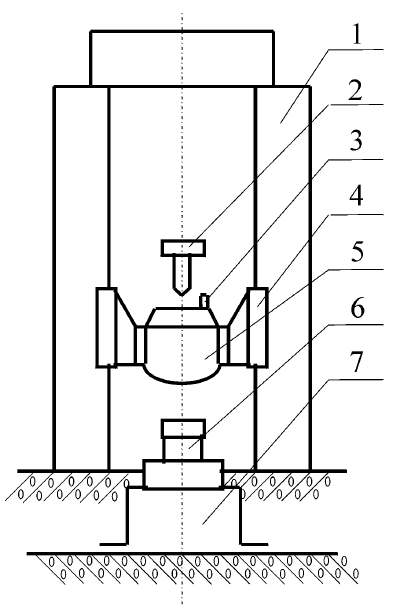
\includegraphics[width=4cm]{cn_100t.png} \\
    1.立柱 2.提升释放机构 3.标准冲击加速度计 \\
    4.导轨 5.重锤 6.被校力传感器 7.底座 \\
  \bicaption[出现在插图索引中]
    {单个图形示例\cite{he1999}。如果表格的标题很长,那么在表格索引中就会很不美观。可
      以在前面用中括号写一个简短的标题,这个标题会出现在索引中。}
    {Stay hungry, stay foolish.}
 \label{fig:cn_100t}
\end{figure}

Lorem ipsum dolor sit amet, consectetur adipisici elit, sed do eiusmod tempor
incididunt ut labore et dolore magna aliqua. Ut enim ad minim veniam, quis
nostrud exercitation ullamco laboris nisi ut aliquip ex ea commodo consequat.
Duis aute irure dolor in reprehenderit in voluptate velit esse cillum dolore eu
fugiat nulla pariatur. Excepteur sint occaecat cupidatat non proident, sunt in
culpa qui officia deserunt mollit anim id est laborum.

\subsection{多个图形}

简单插入多个图形的例子如图~\ref{fig:SRR} 所示。这两个水平并列放置的子图共用一个
图形计数器,没有各自的子图题。

\begin{figure}[!htp]
  \centering
  
\includegraphics[height=2cm]{sjtu-vi-badge-blue.pdf}
  \hspace{1cm}
  
\includegraphics[height=2cm]{sjtu-vi-badge-blue.pdf}
  \bicaption{中文题图}{English caption}
  \label{fig:SRR}
\end{figure}

如果多个图形相互独立,并不共用一个图形计数器,那么用 \texttt{minipage} 或者
\texttt{parbox} 就可以,如图~\ref{fig:parallel1} 与图~\ref{fig:parallel2}。

\begin{figure}[!htp]
\begin{minipage}{0.48\textwidth}
  \centering
  
\includegraphics[height=1.5cm]{sjtu-vi-name-blue.pdf}
  \caption{并排第一个图}
  \label{fig:parallel1}
\end{minipage}\hfill
\begin{minipage}{0.48\textwidth}
  \centering
  
\includegraphics[height=1.5cm]{sjtu-vi-name-blue.pdf}
  \caption{并排第二个图}
  \label{fig:parallel2}
\end{minipage}
\end{figure}

Lorem ipsum dolor sit amet, consectetur adipisici elit, sed do eiusmod tempor
incididunt ut labore et dolore magna aliqua. Ut enim ad minim veniam, quis
nostrud exercitation ullamco laboris nisi ut aliquip ex ea commodo consequat.
Duis aute irure dolor in reprehenderit in voluptate velit esse cillum dolore eu
fugiat nulla pariatur. Excepteur sint occaecat cupidatat non proident, sunt in
culpa qui officia deserunt mollit anim id est laborum.

如果要为共用一个计数器的多个子图添加子图题,建议使用较新的 \pkg{subcaption}宏
包,不建议使用 \pkg{subfigure} 或 \pkg{subfig} 等宏包。

推荐使用 \pkg{subcaption} 宏包的 \cs{subcaptionbox} 并排子图,子图题置于子图之
下,子图号用 a)、b) 等表示。也可以使用 \pkg{subcaption} 宏包的 \cs{subcaption}
(放在 minipage中,用法同 \cs{caption})。

搭配 \pkg{bicaption} 宏包时,可以启用 \cs{subcaptionbox} 和 \cs{subcaption} 的双
语变种 \cs{bisubcaptionbox} 和 \cs{bisubcaption},如图~\ref{fig:bisubcaptionbox}
所示。

\begin{figure}[!hbtp]
  \centering
  \bisubcaptionbox{$R_3 = 1.5\text{mm}$ 时轴承的压力分布云图}%
                  {Pressure contour of bearing when $R_3 = 1.5\text{mm}$}%
                  [6.4cm]{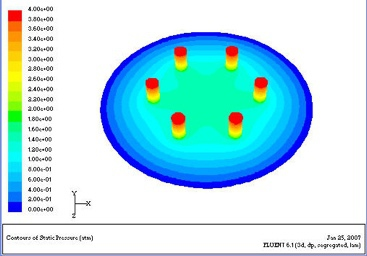
\includegraphics[height=2.5cm]{pressure15.jpg}}
  \hspace{1cm}
  \bisubcaptionbox{$R_3 = 2.5\text{mm}$ 时轴承的压力分布云图}%
                  {Pressure contour of bearing when $R_3 = 2.5\text{mm}$}%
                  [6.4cm]{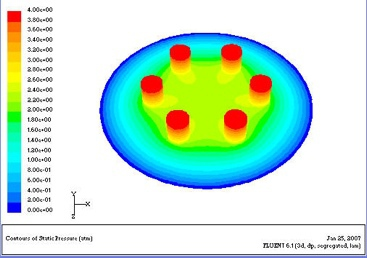
\includegraphics[height=2.5cm]{/pressure25.jpg}}
  \bicaption{包含子图题的范例(使用 subcaptionbox)}
            {Example with subcaptionbox}
  \label{fig:bisubcaptionbox}
\end{figure}

\pkg{subcaption} 宏包也提供了 \pkg{subfigure} 和 \pkg{subtable} 环境,如
图~\ref{fig:subfigure}。

\begin{figure}[!htp]
  \centering
  \begin{subfigure}{0.3\textwidth}
    \centering
    
\includegraphics[height=2cm]{sjtu-vi-badge-blue.pdf}
    \caption{校徽}
  \end{subfigure}
  \hspace{1cm}
  \begin{subfigure}{0.4\textwidth}
    \centering
    
\includegraphics[height=1.5cm]{sjtu-vi-name-blue.pdf}
    \caption{校名。注意这个图略矮些,subfigure 中同一行的子图在顶端对齐。}
  \end{subfigure}
  \caption{包含子图题的范例(使用 subfigure)}
  \label{fig:subfigure}
\end{figure}

Lorem ipsum dolor sit amet, consectetur adipisici elit, sed do eiusmod tempor
incididunt ut labore et dolore magna aliqua. Ut enim ad minim veniam, quis
nostrud exercitation ullamco laboris nisi ut aliquip ex ea commodo consequat.
Duis aute irure dolor in reprehenderit in voluptate velit esse cillum dolore eu
fugiat nulla pariatur. Excepteur sint occaecat cupidatat non proident, sunt in
culpa qui officia deserunt mollit anim id est laborum.

\section{表格}

\subsection{基本表格}

编排表格应简单明了,表达一致,明晰易懂,表文呼应、内容一致。表题置于表上,研究生
学位论文可以用中、英文两种文字居中排写,中文在上,也可以只用中文。

表格的编排建议采用国际通行的三线表\footnote{三线表,以其形式简洁、功能分明、阅读
方便而在科技论文中被推荐使用。三线表通常只有 3 条线,即顶线、底线和栏目线,没有
竖线。}。三线表可以使用 \pkg{booktabs} 提供的 \cs{toprule}、\cs{midrule} 和
\cs{bottomrule}。它们与 \pkg{longtable} 能很好的配合使用。

\begin{table}[!hpt]
  \caption[一个颇为标准的三线表]{一个颇为标准的三线表\footnotemark}
  \label{tab:firstone}
  \centering
  \begin{tabular}{@{}llr@{}} \toprule
    \multicolumn{2}{c}{Item} \\ \cmidrule(r){1-2}
    Animal & Description & Price (\$)\\ \midrule
    Gnat  & per gram  & 13.65 \\
          & each      & 0.01 \\
    Gnu   & stuffed   & 92.50 \\
    Emu   & stuffed   & 33.33 \\
    Armadillo & frozen & 8.99 \\ \bottomrule
  \end{tabular}
\end{table}
\footnotetext{这个例子来自
  \href{https://mirrors.sjtug.sjtu.edu.cn/ctan/macros/latex/contrib/booktabs/booktabs.pdf}%
  {《Publication quality tables in LaTeX》}(\pkg{booktabs} 宏包的文档)。这也是
  一个在表格中使用脚注的例子,请留意与 \pkg{threeparttable} 实现的效果有何不
  同。}

\subsection{复杂表格}

我们经常会在表格下方标注数据来源,或者对表格里面的条目进行解释。可以用
\pkg{threeparttable} 实现带有脚注的表格,如表~\ref{tab:footnote}。

\begin{table}[!htpb]
  \bicaption{一个带有脚注的表格的例子}{A Table with footnotes}
  \label{tab:footnote}
  \centering
  \begin{threeparttable}[b]
     \begin{tabular}{ccd{4}cccc}
      \toprule
      \multirow{2}*{total} & \multicolumn{2}{c}{20\tnote{a}} & \multicolumn{2}{c}{40} & \multicolumn{2}{c}{60} \\
      \cmidrule(lr){2-3}\cmidrule(lr){4-5}\cmidrule(lr){6-7}
      & www & \multicolumn{1}{c}{k} & www & k & www & k \\ % 使用说明符 d 的列会自动进入数学模式,使用 \multicolumn 对文字表头做特殊处理
      \midrule
      & $\underset{(2.12)}{4.22}$ & 120.0140\tnote{b} & 333.15 & 0.0411 & 444.99 & 0.1387 \\
      & 168.6123 & 10.86 & 255.37 & 0.0353 & 376.14 & 0.1058 \\
      & 6.761    & 0.007 & 235.37 & 0.0267 & 348.66 & 0.1010 \\
      \bottomrule
    \end{tabular}
    \begin{tablenotes}
    \item [a] the first note.% or \item [a]
    \item [b] the second note.% or \item [b]
    \end{tablenotes}
  \end{threeparttable}
\end{table}

Lorem ipsum dolor sit amet, consectetur adipisici elit, sed do eiusmod tempor
incididunt ut labore et dolore magna aliqua. Ut enim ad minim veniam, quis
nostrud exercitation ullamco laboris nisi ut aliquip ex ea commodo consequat.
Duis aute irure dolor in reprehenderit in voluptate velit esse cillum dolore eu
fugiat nulla pariatur. Excepteur sint occaecat cupidatat non proident, sunt in
culpa qui officia deserunt mollit anim id est laborum.

如某个表需要转页接排,可以用 \pkg{longtable} 实现。接排时表题省略,表头应重复书
写,并在右上方写“续表 xx”,如表~\ref{tab:performance}。

\begin{ThreePartTable}
  \begin{TableNotes}
    \item[a] 一个脚注
    \item[b] 另一个脚注
  \end{TableNotes}
  \begin{longtable}[c]{c*{6}{r}}
    \bicaption{实验数据}{Experimental data}
    \label{tab:performance} \\
    \toprule
    测试程序 & \multicolumn{1}{c}{正常运行} & \multicolumn{1}{c}{同步}
      & \multicolumn{1}{c}{检查点} & \multicolumn{1}{c}{卷回恢复}
      & \multicolumn{1}{c}{进程迁移} & \multicolumn{1}{c}{检查点} \\
    & \multicolumn{1}{c}{时间 (s)} & \multicolumn{1}{c}{时间 (s)}
      & \multicolumn{1}{c}{时间 (s)} & \multicolumn{1}{c}{时间 (s)}
      & \multicolumn{1}{c}{时间 (s)} &  文件(KB)\\
    \midrule
    \endfirsthead
    \multicolumn{7}{r}{续表~\thetable} \\
    \toprule
    测试程序 & \multicolumn{1}{c}{正常运行} & \multicolumn{1}{c}{同步}
      & \multicolumn{1}{c}{检查点} & \multicolumn{1}{c}{卷回恢复}
      & \multicolumn{1}{c}{进程迁移} & \multicolumn{1}{c}{检查点} \\
    & \multicolumn{1}{c}{时间 (s)} & \multicolumn{1}{c}{时间 (s)}
      & \multicolumn{1}{c}{时间 (s)} & \multicolumn{1}{c}{时间 (s)}
      & \multicolumn{1}{c}{时间 (s)}&  文件(KB)\\
    \midrule
    \endhead
    \hline
    \multicolumn{7}{r}{续下页}
    \endfoot
    \insertTableNotes
    \endlastfoot
    CG.A.2 & 23.05 & 0.002 & 0.116 & 0.035 & 0.589 & 32491 \\
    CG.A.4 & 15.06 & 0.003 & 0.067 & 0.021 & 0.351 & 18211 \\
    CG.A.8 & 13.38 & 0.004 & 0.072 & 0.023 & 0.210 & 9890 \\
    CG.B.2 & 867.45 & 0.002 & 0.864 & 0.232 & 3.256 & 228562 \\
    CG.B.4 & 501.61 & 0.003 & 0.438 & 0.136 & 2.075 & 123862 \\
    CG.B.8 & 384.65 & 0.004 & 0.457 & 0.108 & 1.235 & 63777 \\
    MG.A.2 & 112.27 & 0.002 & 0.846 & 0.237 & 3.930 & 236473 \\
    MG.A.4 & 59.84 & 0.003 & 0.442 & 0.128 & 2.070 & 123875 \\
    MG.A.8 & 31.38 & 0.003 & 0.476 & 0.114 & 1.041 & 60627 \\
    MG.B.2 & 526.28 & 0.002 & 0.821 & 0.238 & 4.176 & 236635 \\
    MG.B.4 & 280.11 & 0.003 & 0.432 & 0.130 & 1.706 & 123793 \\
    MG.B.8 & 148.29 & 0.003 & 0.442 & 0.116 & 0.893 & 60600 \\
    LU.A.2 & 2116.54 & 0.002 & 0.110 & 0.030 & 0.532 & 28754 \\
    LU.A.4 & 1102.50 & 0.002 & 0.069 & 0.017 & 0.255 & 14915 \\
    LU.A.8 & 574.47 & 0.003 & 0.067 & 0.016 & 0.192 & 8655 \\
    LU.B.2 & 9712.87 & 0.002 & 0.357 & 0.104 & 1.734 & 101975 \\
    LU.B.4 & 4757.80 & 0.003 & 0.190 & 0.056 & 0.808 & 53522 \\
    LU.B.8 & 2444.05 & 0.004 & 0.222 & 0.057 & 0.548 & 30134 \\
    EP.A.2 & 123.81 & 0.002 & 0.010 & 0.003 & 0.074 & 1834 \\
    EP.A.4 & 61.92 & 0.003 & 0.011 & 0.004 & 0.073 & 1743 \\
    EP.A.8 & 31.06 & 0.004 & 0.017 & 0.005 & 0.073 & 1661 \\
    EP.B.2 & 495.49 & 0.001 & 0.009 & 0.003 & 0.196 & 2011 \\
    EP.B.4 & 247.69 & 0.002 & 0.012 & 0.004 & 0.122 & 1663 \\
    EP.B.8 & 126.74 & 0.003 & 0.017 & 0.005 & 0.083 & 1656 \\
    SP.A.2 & 123.81 & 0.002 & 0.010 & 0.003 & 0.074 & 1854 \\
    SP.A.4 & 51.92 & 0.003 & 0.011 & 0.004 & 0.073 & 1543 \\
    SP.A.8 & 31.06 & 0.004 & 0.017 & 0.005 & 0.073 & 1671 \\
    SP.B.2 & 495.49 & 0.001 & 0.009 & 0.003 & 0.196 & 2411 \\
    SP.B.4 \tnote{a} & 247.69 & 0.002 & 0.014 & 0.006 & 0.152 & 2653 \\
    SP.B.8 \tnote{b} & 126.74 & 0.003 & 0.017 & 0.005 & 0.082 & 1755 \\
    \bottomrule
  \end{longtable}
\end{ThreePartTable}

\section{算法环境}

算法环境可以使用 \pkg{algorithms} 宏包或者较新的 \pkg{algorithm2e} 实现。
算法~\ref{algo:algorithm} 是一个使用 \pkg{algorithm2e} 的例子。关于排版算法环境
的具体方法,请阅读相关宏包的官方文档。

\begin{algorithm}[htb]
  \caption{算法示例}
  \label{algo:algorithm}
  \small
  \SetAlgoLined
  \KwData{this text}
  \KwResult{how to write algorithm with \LaTeXe }

  initialization\;
  \While{not at end of this document}{
    read current\;
    \eIf{understand}{
      go to next section\;
      current section becomes this one\;
    }{
      go back to the beginning of current section\;
    }
  }
\end{algorithm}

\section{代码环境}

我们可以在论文中插入算法,但是不建议插入大段的代码。如果确实需要插入代码,建议使
用 \pkg{listings} 宏包。

\begin{codeblock}[language=C]
#include <stdio.h>
#include <unistd.h>
#include <sys/types.h>
#include <sys/wait.h>

int main() {
  pid_t pid;

  switch ((pid = fork())) {
  case -1:
    printf("fork failed\n");
    break;
  case 0:
    /* child calls exec */
    execl("/bin/ls", "ls", "-l", (char*)0);
    printf("execl failed\n");
    break;
  default:
    /* parent uses wait to suspend execution until child finishes */
    wait((int*)0);
    printf("is completed\n");
    break;
  }

  return 0;
}
\end{codeblock}

\section{目录树环境}
可以在正文中用dirtree包来表示代码目录树,还有一种做法是先在代码目录下用tree命令打印目录树再以文本形式复制到正文中。每一行表示一个条目,可以是文件或文件夹,第一个序号表示当前的条目的目录树深度,随后是条目名称,每一行以.结尾。还有三个特殊命令(1)\DTstyle:定义节点文本的命令,当你在LATEX中它的默认值是\ttfamily。在TeX中默认值是\tt,可以重定义这个命令(2)\DTcomment:允许将文本放在某一级右侧,用法是:\DTcomment{comment text}(3)\DTstylecomment:右侧文本的风格用这个命令用来定义,在LATEX下默认值是\rmfamilly ,TeX中默认值是\rm。一个综合上述三个命令的例子:
\renewcommand*\DTstylecomment{\rmfamily\color{green}\textsc} \renewcommand*\DTstyle{\ttfamily\textcolor{red}} 
\dirtree{%
.1 /. 
.2 bin.
.2 home. 
.3 jeancome. 
.4 texmf.
.5 tex.
.3 jeancomeson\DTcomment{Guillaume}. 
.3 jeancomedaughter\DTcomment{Mathilde}. 
.2 usr.
.3 bin.
}

% !TEX root = ../thesis.tex

\chapter{数学与引用文献的标注}

\section{数学}

\subsection{数字和单位}

宏包 \pkg{siunitx} 提供了更好的数字和单位支持:
\begin{itemize}
  \item \num{12345.67890}
  \item \num{1+-2i}
  \item \num{.3e45}
  \item \num{1.654 x 2.34 x 3.430}
  \item \si{kg.m.s^{-1}}
  \item \si{\micro\meter} $\si{\micro\meter}$
  \item \si{\ohm} $\si{\ohm}$
  \item \numlist{10;20}
  \item \numlist{10;20;30}
  \item \SIlist{0.13;0.67;0.80}{\milli\metre}
  \item \numrange{10}{20}
  \item \SIrange{10}{20}{\degreeCelsius}
\end{itemize}

\subsection{数学符号和公式}

微分符号 $\dif$ 应使用正体,本模板提供了 \cs{dif} 命令。除此之外,模板还提供了一
些命令方便使用:
\begin{itemize}
  \item 圆周率 $\uppi$:\verb|\uppi|
  \item 自然对数的底 $\upe$:\verb|\upe|
  \item 虚数单位 $\upi$, $\upj$:\verb|\upi| \verb|\upj|
\end{itemize}

公式应另起一行居中排版。公式后应注明编号,按章顺序编排,编号右端对齐。
\begin{equation}
  \upe^{\upi\uppi} + 1 = 0,
\end{equation}
\begin{equation}
  \frac{\dif^2 u}{\dif t^2} = \int f(x) \dif x.
\end{equation}

公式末尾是需要添加标点符号的,至于用逗号还是句号,取决于公式下面一句是接着公式说的,还是另起一句。
\begin{equation}
		\frac{2h}{\pi}\int_{0}^{\infty}\frac{\sin\left( \omega\delta \right)}{\omega}
		\cos\left( \omega x \right) \dif\omega = 
		\begin{cases}
				h, \ \left| x \right| < \delta, \\
				\frac{h}{2}, \ x = \pm \delta, \\
				0, \ \left| x \right| > \delta.
		\end{cases}
\end{equation}
公式较长时最好在等号“$=$”处转行。
\begin{align}
    & I (X_3; X_4) - I (X_3; X_4 \mid X_1) - I (X_3; X_4 \mid X_2) \nonumber \\
  = & [I (X_3; X_4) - I (X_3; X_4 \mid X_1)] - I (X_3; X_4 \mid \tilde{X}_2) \\
  = & I (X_1; X_3; X_4) - I (X_3; X_4 \mid \tilde{X}_2).
\end{align}

如果在等号处转行难以实现,也可在 $+$、$-$、$\times$、$\div$运算符号处转行,转行
时运算符号仅书写于转行式前,不重复书写。
\begin{multline}
  \frac{1}{2} \Delta (f_{ij} f^{ij}) =
    2 \left(\sum_{i<j} \chi_{ij}(\sigma_{i} - \sigma_{j})^{2}
    + f^{ij} \nabla_{j} \nabla_{i} (\Delta f) \right. \\
  \left. + \nabla_{k} f_{ij} \nabla^{k} f^{ij} +
    f^{ij} f^{k} \left[2\nabla_{i}R_{jk}
    - \nabla_{k} R_{ij} \right] \vphantom{\sum_{i<j}} \right).
\end{multline}

\subsection{定理环境}

示例文件中使用 \pkg{ntheorem} 宏包配置了定理、引理和证明等环境。用户也可以使用
\pkg{amsthm} 宏包。

这里举一个“定理”和“证明”的例子。
\begin{theorem}[留数定理]
\label{thm:res}
  假设 $U$ 是复平面上的一个单连通开子集,$a_1, \ldots, a_n$ 是复平面上有限个点,
  $f$ 是定义在 $U \backslash \{a_1, \ldots, a_n\}$ 上的全纯函数,如果 $\gamma$
  是一条把 $a_1, \ldots, a_n$ 包围起来的可求长曲线,但不经过任何一个 $a_k$,并且
  其起点与终点重合,那么:

  \begin{equation}
    \label{eq:res}
    \ointop_\gamma f(z)\, \dif z = 2\uppi \upi \sum_{k=1}^n \operatorname{I}(\gamma, a_k) \operatorname{Res}(f, a_k).
  \end{equation}

  如果 $\gamma$ 是若尔当曲线,那么 $\operatorname{I}(\gamma, a_k) = 1$,因此:

  \begin{equation}
    \label{eq:resthm}
    \ointop_\gamma f(z)\, \dif z = 2\uppi \upi \sum_{k=1}^n \operatorname{Res}(f, a_k).
  \end{equation}

  在这里,$\operatorname{Res}(f, a_k)$ 表示 $f$ 在点 $a_k$ 的留数,
  $\operatorname{I}(\gamma, a_k)$ 表示 $\gamma$ 关于点 $a_k$ 的卷绕数。卷绕数是
  一个整数,它描述了曲线 $\gamma$ 绕过点 $a_k$ 的次数。如果 $\gamma$ 依逆时针方
  向绕着 $a_k$ 移动,卷绕数就是一个正数,如果 $\gamma$ 根本不绕过 $a_k$,卷绕数
  就是零。

  定理~\ref{thm:res} 的证明。

  \begin{proof}
    首先,由……

    其次,……

    所以……
  \end{proof}
\end{theorem}

\section{引用文献的标注}

按照教务处的要求,参考文献外观应符合国标 GB/T 7714 的要求。模版使用 \BibLaTeX\
配合 \pkg{biblatex-gb7714-2015} 样式包
\footnote{\url{https://www.ctan.org/pkg/biblatex-gb7714-2015}}
控制参考文献的输出样式,后端采用 \pkg{biber} 管理文献。

请注意 \pkg{biblatex-gb7714-2015} 宏包 2016 年 9 月才加入 CTAN,如果你使用的
\TeX\ 系统版本较旧,可能没有包含 \pkg{biblatex-gb7714-2015} 宏包,需要手动安装。
\BibLaTeX\ 与 \pkg{biblatex-gb7714-2015} 目前在活跃地更新,为避免一些兼容性问
题,推荐使用较新的版本。

正文中引用参考文献时,使用 \verb|\cite{key1,key2,key3...}| 可以产生“上标引用的
参考文献”,如 \cite{Meta_CN,chen2007act,DPMG}。使用
\verb|\parencite{key1,key2,key3...}| 则可以产生水平引用的参考文献,例如
\parencite{JohnD,zhubajie,IEEE-1363}。请看下面的例子,将会穿插使用水平的和上标的
参考文献:关于书的\parencite{Meta_CN,JohnD,IEEE-1363},关于期刊的
\cite{chen2007act,chen2007ewi},会议论文 \parencite{DPMG,kocher99,cnproceed},硕
士学位论文\parencite{zhubajie,metamori2004},博士学位论文
\cite{shaheshang,FistSystem01,bai2008},标准文件 \parencite{IEEE-1363},技术报告
\cite{NPB2},电子文献 \parencite{xiaoyu2001, CHRISTINE1998},用户手册
\parencite{RManual}。

当需要将参考文献条目加入到文献表中但又不在正文中引用,可以使用
\verb|\nocite{key1,key2,key3...}|。使用 \verb|\nocite{*}| 可以将参考文献数据库中
的所有条目加入到文献表中。

% !TEX root = ../thesis.tex

\begin{summary}
这里是全文总结内容。

2015 年 2 月 28 日,中央在北京召开全国精神文明建设工作表彰暨学雷锋志愿服务大会,
公布全国文明城市(区)、文明村镇、文明单位名单。上海交通大学荣获全国文明单位称
号。

全国文明单位这一荣誉是对交大人始终高度重视文明文化工作的肯定,是对交大长期以来文
明创建工作成绩的褒奖。在学校党委、文明委的领导下,交大坚持将文明创建工作纳入学校
建设世界一流大学的工作中,全体师生医护员工群策群力、积极开拓,落实国家和上海市有
关文明创建的各项要求,以改革创新、科学发展为主线,以质量提升为目标,聚焦文明创建
工作出现的重点和难点,优化文明创建工作机制,传播学校良好形象,提升社会美誉度,显
著增强学校软实力。2007 至 2012 年间,上海交大连续三届荣获“上海市文明单位”称
号,成为创建全国文明单位的新起点。

上海交大自启动争创全国文明单位工作以来,凝魂聚气、改革创新,积极培育和践行社会主
义核心价值观。坚持统筹兼顾、多措并举,将争创全国文明单位与学校各项中心工作紧密结
合,着力构建学校文明创建新格局,不断提升师生医护员工文明素养,以“冲击世界一流大
学汇聚强大精神动力”为指导思想,以“聚焦改革、多元推进、以评促建、丰富内涵、彰显
特色”为工作原则,并由全体校领导群策领衔“党的建设深化、思想教育深入、办学成绩显
著、大学文化丰富、校园环境优化、社会责任担当”六大板块共 28 项重点突破工作,全面
展现近年来交大文明创建工作的全貌和成就。

进入新阶段,学校将继续开拓文明创建工作新格局,不断深化工作理念和工作实践,创新工
作载体、丰富活动内涵、凸显创建成效,积极服务于学校各项中心工作和改革发展的大局
面,在上级党委、文明委的关心下,在学校党委的直接领导下,与时俱进、开拓创新,为深
化内涵建设、加快建成世界一流大学、推动国家进步和社会发展而努力奋斗!

上海交通大学医学院附属仁济医院也获得全国文明单位称号。
\end{summary}


% 使用英文字母对附录编号
\appendix

% 附录内容,本科学位论文可以用翻译的文献替代。
% !TEX root = ../main.tex

\chapter{Maxwell Equations}

选择二维情况,有如下的偏振矢量:
\begin{subequations}
  \begin{align}
    {\bf E} &= E_z(r, \theta) \hat{\bf z}, \\
    {\bf H} &= H_r(r, \theta) \hat{\bf r} + H_\theta(r, \theta) \hat{\bm\theta}.
  \end{align}
\end{subequations}
对上式求旋度:
\begin{subequations}
  \begin{align}
    \nabla \times {\bf E} &= \frac{1}{r} \frac{\partial E_z}{\partial\theta}
      \hat{\bf r} - \frac{\partial E_z}{\partial r} \hat{\bm\theta}, \\
    \nabla \times {\bf H} &= \left[\frac{1}{r} \frac{\partial}{\partial r}
      (r H_\theta) - \frac{1}{r} \frac{\partial H_r}{\partial\theta} \right]
      \hat{\bf z}.
  \end{align}
\end{subequations}
因为在柱坐标系下,$\overline{\overline\mu}$ 是对角的,所以 Maxwell 方程组中电场
$\bf E$ 的旋度:
\begin{subequations}
  \begin{align}
    & \nabla \times {\bf E} = \ii \omega {\bf B}, \\
    & \frac{1}{r} \frac{\partial E_z}{\partial\theta} \hat{\bf r} -
      \frac{\partial E_z}{\partial r}\hat{\bm\theta} = \ii \omega \mu_r H_r
      \hat{\bf r} + \ii \omega \mu_\theta H_\theta \hat{\bm\theta}.
  \end{align}
\end{subequations}
所以 $\bf H$ 的各个分量可以写为:
\begin{subequations}
  \begin{align}
    H_r &= \frac{1}{\ii \omega \mu_r} \frac{1}{r}
      \frac{\partial E_z}{\partial\theta}, \\
    H_\theta &= -\frac{1}{\ii \omega \mu_\theta}
      \frac{\partial E_z}{\partial r}.
  \end{align}
\end{subequations}
同样地,在柱坐标系下,$\overline{\overline\epsilon}$ 是对角的,所以 Maxwell 方程
组中磁场 $\bf H$ 的旋度:
\begin{subequations}
  \begin{align}
    & \nabla \times {\bf H} = -\ii \omega {\bf D}, \\
    & \left[\frac{1}{r} \frac{\partial}{\partial r}(r H_\theta) - \frac{1}{r}
      \frac{\partial H_r}{\partial\theta} \right] \hat{\bf z} = -\ii \omega
      {\overline{\overline\epsilon}} {\bf E} = -\ii \omega \epsilon_z E_z
      \hat{\bf z}, \\
    & \frac{1}{r} \frac{\partial}{\partial r}(r H_\theta) - \frac{1}{r}
      \frac{\partial H_r}{\partial\theta} = -\ii \omega \epsilon_z E_z.
  \end{align}
\end{subequations}
由此我们可以得到关于 $E_z$ 的波函数方程:
\begin{equation}
  \frac{1}{\mu_\theta \epsilon_z} \frac{1}{r} \frac{\partial}{\partial r}
  \left(r \frac{\partial E_z}{\partial r} \right) + \frac{1}{\mu_r \epsilon_z}
  \frac{1}{r^2} \frac{\partial^2E_z}{\partial\theta^2} +\omega^2 E_z = 0.
\end{equation}

% !TEX root = ../thesis.tex

\chapter{绘制流程图}

图~\ref{fig:flow_chart} 是一张流程图示意。使用 \pkg{tikz} 环境,搭配四种预定义节
点(\verb+startstop+、\verb+process+、\verb+decision+和\verb+io+),可以容易地绘
制出流程图。

\begin{figure}[!htp]
  \centering
  \resizebox{6cm}{!}{\begin{tikzpicture}[node distance=2cm]
    \node (pic) [startstop] {待测图片};
    \node (bg) [io, below of=pic] {读取背景};
    \node (pair) [process, below of=bg] {匹配特征点对};
    \node (threshold) [decision, below of=pair, yshift=-0.5cm] {多于阈值};
    \node (clear) [decision, right of=threshold, xshift=3cm] {清晰?};
    \node (capture) [process, right of=pair, xshift=3cm, yshift=0.5cm] {重采};
    \node (matrix_p) [process, below of=threshold, yshift=-0.8cm] {透视变换矩阵};
    \node (matrix_a) [process, right of=matrix_p, xshift=3cm] {仿射变换矩阵};
    \node (reg) [process, below of=matrix_p] {图像修正};
    \node (return) [startstop, below of=reg] {配准结果};
     
    %连接具体形状
    \draw [arrow](pic) -- (bg);
    \draw [arrow](bg) -- (pair);
    \draw [arrow](pair) -- (threshold);

    \draw [arrow](threshold) -- node[anchor=south] {否} (clear);

    \draw [arrow](clear) -- node[anchor=west] {否} (capture);
    \draw [arrow](capture) |- (pic);
    \draw [arrow](clear) -- node[anchor=west] {是} (matrix_a);
    \draw [arrow](matrix_a) |- (reg);

    \draw [arrow](threshold) -- node[anchor=east] {是} (matrix_p);
    \draw [arrow](matrix_p) -- (reg);
    \draw [arrow](reg) -- (return);
\end{tikzpicture}
}
  \bicaption{绘制流程图效果}{Flow chart}
  \label{fig:flow_chart}
\end{figure}


% 文后无编号部分
\backmatter

% 参考资料
\printbibliography[heading=bibintoc]

% 用于盲审的论文需隐去致谢、发表论文、参与项目、申请专利、简历

% 致谢
% !TEX root = ../main.tex

%TC:ignore

\begin{acknowledgements}
  感谢那位最先制作出博士学位论文 \LaTeX 模板的交大物理系同学!

  感谢 William Wang 同学对模板移植做出的巨大贡献!

  感谢 \href{https://github.com/weijianwen}{@weijianwen} 学长一直以来的开发和维
  护工作!

  感谢 \href{https://github.com/sjtug}{@sjtug} 以及
   \href{https://github.com/dyweb}{@dyweb} 对 0.9.5 之后版本的开发和维护工作!

  感谢所有为模板贡献过代码的同学们, 以及所有测试和使用模板的各位同学!

  感谢 \LaTeX 和 \href{https://github.com/sjtug/SJTUThesis}{\sjtuthesis},帮我节
  省了不少时间。
\end{acknowledgements}

%TC:endignore


% 发表论文、参与项目、申请专利、简历
% 盲审论文中,发表学术论文及参与科研情况等仅以第几作者注明即可,不要出现作者或他人姓名
% !TEX root = ../main.tex

\begin{publications}
	\begin{refsection}
		\nocite{jiang2008reflections,chen2007act,chen2007ewi}
		\printbibliography[heading=none]
	\end{refsection}
\end{publications}

\begin{publications*}
	\item 第一作者. 上海交通大学学报, 2008.
	\item 第一作者. 中文核心期刊论文, 2007.
	\item 第一作者. EI 国际会议论文, 2006.
\end{publications*}

% !TEX root = ../thesis.tex

%TC:ignore

\begin{projects}
  \item 参与973项目子课题(2007年6月--2008年5月)
  \item 参与自然基金项目(2005年5月--2005年8月)
  \item 参与国防项目(2005年8月--2005年10月)
\end{projects}

\begin{projects*}
  \item 973项目“XXX”
  \item 自然基金项目“XXX”
  \item 国防项目“XXX”
\end{projects*}

%TC:endignore

% !TEX root = ../thesis.tex

%TC:ignore

\begin{patents}
  \item 第一发明人,“永动机”,专利申请号202510149890.0
\end{patents}

\begin{patents*}
  \item 第一发明人,“永动机”,专利申请号XXXXXXXXXXXX.X
\end{patents*}

%TC:endignore

% !TEX root = ../main.tex

%TC:ignore

\begin{resume}
  \subsection*{基本情况}
    某某,yyyy 年 mm 月生于 xxxx。

  \subsection*{教育背景}
  \begin{itemize}
    \item yyyy 年 mm 月至今,上海交通大学,博士研究生,xx 专业
    \item yyyy 年 mm 月至 yyyy 年 mm 月,上海交通大学,硕士研究生,xx 专业
    \item yyyy 年 mm 月至 yyyy 年 mm 月,上海交通大学,本科,xx 专业
  \end{itemize}

  \subsection*{研究兴趣}
    \LaTeX{} 排版

  \subsection*{联系方式}
  \begin{itemize}
    \item 地址: 上海市闵行区东川路 800 号,200240
    \item E-mail: \email{xxx@sjtu.edu.cn}
  \end{itemize}
\end{resume}

%TC:endignore


% 中文学士学位论文要求在最后有一个英文大摘要,单独编页码,英文学士学位论文不需要
% !TEX root = ../thesis.tex

\begin{bigabstract}
  An imperial edict issued in 1896 by Emperor Guangxu, established Nanyang
  Public School in Shanghai. The normal school, school of foreign studies,
  middle school and a high school were established. Sheng Xuanhuai, the person
  responsible for proposing the idea to the emperor, became the first president
  and is regarded as the founder of the university.

  During the 1930s, the university gained a reputation of nurturing top
  engineers. After the foundation of People's Republic, some faculties were
  transferred to other universities. A significant amount of its faculty were
  sent in 1956, by the national government, to Xi'an to help build up Xi'an Jiao
  Tong University in western China. Afterwards, the school was officially
  renamed Shanghai Jiao Tong University.

  Since the reform and opening up policy in China, SJTU has taken the lead in
  management reform of institutions for higher education, regaining its vigor
  and vitality with an unprecedented momentum of growth. SJTU includes five
  beautiful campuses, Xuhui, Minhang, Luwan Qibao, and Fahua, taking up an area
  of about 3,225,833 m2. A number of disciplines have been advancing towards the
  top echelon internationally, and a batch of burgeoning branches of learning
  have taken an important position domestically.

  Today SJTU has 31 schools (departments), 63 undergraduate programs, 250
  masters-degree programs, 203 Ph.D. programs, 28 post-doctorate programs, and
  11 state key laboratories and national engineering research centers.

  SJTU boasts a large number of famous scientists and professors, including 35
  academics of the Academy of Sciences and Academy of Engineering, 95 accredited
  professors and chair professors of the "Cheung Kong Scholars Program" and more
  than 2,000 professors and associate professors.

  Its total enrollment of students amounts to 35,929, of which 1,564 are
  international students. There are 16,802 undergraduates, and 17,563 masters
  and Ph.D. candidates. After more than a century of operation, Jiao Tong
  University has inherited the old tradition of "high starting points, solid
  foundation, strict requirements and extensive practice." Students from SJTU
  have won top prizes in various competitions, including ACM International
  Collegiate Programming Contest, International Mathematical Contest in Modeling
  and Electronics Design Contests. Famous alumni include Jiang Zemin, Lu Dingyi,
  Ding Guangen, Wang Daohan, Qian Xuesen, Wu Wenjun, Zou Taofen, Mao Yisheng,
  Cai Er, Huang Yanpei, Shao Lizi, Wang An and many more. More than 200 of the
  academics of the Chinese Academy of Sciences and Chinese Academy of
  Engineering are alumni of Jiao Tong University.
\end{bigabstract}


\end{document}
